\chapter{Solution Design}
\label{chap:SolutionDesign}

\section{Requirements}

\subsection{Functional Requirements}

The solution design focuses on an AI-enabled production order release system with the following key functional requirements:

\begin{itemize}
    \item \textbf{AI-Enabled Case Management}: The system should leverage artificial intelligence to analyze production order descriptions and compare them with historical data to make intelligent release decisions.
    
    \item \textbf{Historical Data Analysis}: The system must fetch and analyze production order information from the past month to identify patterns and similarities in component usage and production requirements.
    
    \item \textbf{Component Availability Checking}: Instead of traditional BOM (Bill of Materials) verification, the system should check past production orders with similar components to assess feasibility.
    
    \item \textbf{ATP (Available-to-Promise) Validation}: The system must perform ATP checks for missing components to ensure production feasibility before order release.
    
    \item \textbf{Intelligent Recommendations}: The system should provide alternative solutions based on past events and historical production data.
    
    \item \textbf{Automated Testing Framework}: Integration with Cucumber framework for comprehensive automated testing of the solution.
\end{itemize}

\subsection{Non-Functional Requirements}

\begin{itemize}
    \item \textbf{Integration Capability}: Seamless integration with SAP S/4HANA Public Cloud Edition
    \item \textbf{Performance}: Real-time processing of production order release decisions
    \item \textbf{Scalability}: Ability to handle multiple production orders simultaneously
    \item \textbf{Reliability}: High availability and fault tolerance
\end{itemize}

\section{System Architecture}

\subsection{Overview}

The solution architecture is designed around a multi-layered approach that integrates AI capabilities with SAP S/4HANA's existing infrastructure. The core components include:

\begin{itemize}
    \item \textbf{Agentic Layer}: Central intelligence unit that processes production orders and makes release decisions
    \item \textbf{Joule Integration}: Independent copilot functionality that provides AI-powered assistance
    \item \textbf{SAP S/4HANA Integration}: Native integration with the existing SAP system for automated production order release via OData APIs
\end{itemize}

\begin{figure}[h]
    \centering
    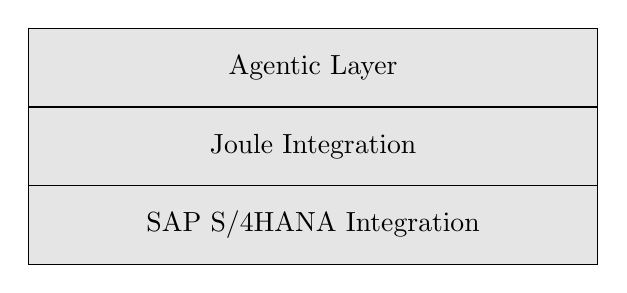
\begin{tikzpicture}[
        layer/.style={rectangle, draw, fill=gray!20, text width=7cm, text centered, minimum height=1cm}
    ]
    
    % Define layers
    \node[layer] (ai) at (0, 2) {Agentic Layer};
    \node[layer] (joule) at (0, 1) {Joule Integration};
    \node[layer] (sap) at (0, 0) {SAP S/4HANA Integration};
    
    \end{tikzpicture}
    \caption{System Architecture Overview}
    \label{fig:system-architecture}
\end{figure}
